\documentclass[lettersize,journal]{IEEEtran}

\usepackage{amsmath,amsfonts,amssymb}
\usepackage{algorithm}
\usepackage{algorithmic}
\usepackage{array}
\usepackage{booktabs}
\usepackage{cite}
\usepackage{graphicx}
\usepackage{url}
\usepackage{xcolor}

\hyphenation{op-tical net-works semi-conduc-tor}

\newcommand{\ind}{\mathbb{I}}
\newcommand{\clip}{\operatorname{clip}}
\newcommand{\cvar}{\operatorname{CVaR}}

\begin{document}

\title{Constraint-Aware Hierarchical Deep Reinforcement Learning for Energy-Efficient Dynamic Edge--Cloud Workflow Scheduling}

\author{% Author information will be inserted before submission.
}

\maketitle

\begin{abstract}
Energy-aware scheduling of dynamically arriving directed-acyclic-graph (DAG)
workflows requires two coupled decisions: assigning each ready task to a
heterogeneous edge or cloud server and selecting its dynamic-voltage-and-frequency-
scaling (DVFS) ratio. A lower frequency may save dynamic power, but it also
extends execution and queue occupancy, thereby increasing the deadline risk of
the current and subsequent workflows. This paper formulates the problem as
computing-energy minimization under workflow-level deadline and reliability
requirements and proposes a constraint-aware hierarchical reinforcement learning
framework. A three-head Dueling Double DQN performs discrete server placement
by separately estimating energy utility, deadline cost, and reliability cost.
Conditioned on the selected server, a Soft Actor--Critic controller determines
a continuous DVFS ratio. Queue-aware dense deadline credit, remaining-critical-
path safety features, episode-level failure feedback, and workflow-level
counterfactual DVFS attribution connect delayed violations to the responsible
upper- and lower-level actions. Separate Lagrangian controllers regulate the
constraint pressure at the two levels. Evaluation uses a constraint-first
protocol: energy is compared only among methods satisfying the prescribed
empirical success probability (ESP) and reliability gates. Across the main
small and medium scenarios, the proposed method attains 95--100\% ESP at a
90\% per-run deadline-satisfaction target and 100\% reliability attainment.
Relative to the lowest-energy feasible baseline, it reduces energy by
22.30--27.70\% in the small scenario and 13.45--20.90\% in the medium scenario.
Ablation results show that continuous DVFS provides an additional 3.31--5.13\%
energy reduction, while removing the upper deadline head collapses ESP to zero.
\end{abstract}

\begin{IEEEkeywords}
Edge--cloud computing, workflow scheduling, deep reinforcement learning,
DVFS, deadline constraint, reliability, Lagrangian optimization.
\end{IEEEkeywords}

\section{Introduction}
\label{sec:introduction}

\IEEEPARstart{D}{ata}-intensive applications in industrial Internet of Things,
scientific analytics, and intelligent services are increasingly represented as
DAG workflows. Edge--cloud platforms can execute these workflows close to data
sources while retaining access to powerful cloud servers. Their heterogeneity,
however, makes online scheduling difficult: a task's finish time depends on its
predecessors, communication, the selected server, and the evolving server queue.
When workflows arrive dynamically, one placement can also delay tasks belonging
to other workflows.

Classical list schedulers such as HEFT provide an effective static baseline for
heterogeneous systems~\cite{topcuoglu2002}, while dynamic workflow methods add
deadline, cost, and multi-workflow awareness~\cite{arabnejad2019,ismayilov2020}.
Deep reinforcement learning (DRL) further enables decisions to adapt to the
current system state~\cite{jayanetti2022,chen2023,pan2024}. Nevertheless, joint
placement and DVFS control remains challenging. Placement is discrete, whereas
the DVFS ratio is continuous. Treating them as a single action obscures their
different physical roles; optimizing them independently ignores their queue-
mediated interaction.

The quality-of-service requirements are also long-horizon constraints rather
than immediate objectives. A workflow can miss its deadline many decisions
after the responsible placement or frequency action. A terminal binary penalty
is therefore too sparse, while a fixed weighted reward has no invariant meaning
when workload size and congestion change. Constrained RL provides adaptive
Lagrangian mechanisms~\cite{achiam2017,tessler2019,stooke2020}, but its use here
still requires a defensible assignment of workflow-level violations to the two
control levels. Reliability introduces another constraint because the transient-
fault rate varies with the operating frequency~\cite{zhang2017,wu2018,hassan2020}.

This paper develops a hierarchical constrained DRL framework for computing-
energy minimization under deadline and reliability requirements. The upper
policy uses three Dueling Double-DQN heads~\cite{vanhasselt2016,wang2016dueling}
to estimate energy, deadline, and reliability consequences for every server.
The lower policy uses SAC~\cite{haarnoja2018} to select a continuous DVFS ratio
after the server is known. The method adds queue-induced dense deadline credit,
remaining-critical-path features, episode-level failure feedback, and a workflow-
level counterfactual replay that measures the delay attributable to DVFS while
holding placements and within-server order fixed.

The main contributions are as follows.
\begin{enumerate}
  \item We formulate online multi-workflow scheduling as a mixed discrete--
  continuous energy-minimization problem with stochastic arrivals, precedence,
  communication, non-preemptive queues, deadlines, and frequency-dependent
  reliability.
  \item We design a three-head upper D3QN and a continuous lower SAC controller,
  with separate constraint signals and Lagrangian controllers instead of one
  fixed multi-objective reward.
  \item We introduce cross-level deadline credit mechanisms that expose queue
  externality to the upper policy and attribute workflow-level delay to lower-
  level DVFS decisions through counterfactual schedule replay.
  \item We use a constraint-first evaluation protocol based on ESP: a method's
  energy is treated as feasible only after its deadline and reliability gates
  are satisfied.
\end{enumerate}
The method targets empirical constraint satisfaction over the workload
distribution; it does not claim a deterministic hard-real-time guarantee for
every unseen arrival sequence.

\section{Related Work}
\label{sec:related_work}

\subsection{Dynamic DAG Workflow Scheduling}
HEFT ranks tasks by their upward ranks and greedily selects the processor with
the earliest finish time~\cite{topcuoglu2002}. It remains a strong reference,
but its original formulation assumes a static workflow. Dynamic multi-workflow
schedulers incorporate arrival time, deadline, and monetary cost
~\cite{arabnejad2019}, while evolutionary methods search for multi-objective
solutions~\cite{ismayilov2020}. These approaches can require repeated planning
as the queue state changes.

DRL replaces repeated combinatorial search with learned online decisions.
Jayanetti \emph{et al.} jointly considered time and energy for precedence-
constrained edge--cloud tasks~\cite{jayanetti2022}. Other studies learn
collaborative heterogeneous-workflow scheduling or real-time cloud scheduling
~\cite{chen2023,pan2024}. Most existing methods, however, use a fixed reward
mixture or a single action type. Our work explicitly separates discrete server
placement from continuous frequency control and couples them through shared
physical and constraint feedback.

\subsection{Constrained and Hierarchical Reinforcement Learning}
Constrained policy optimization~\cite{achiam2017}, reward-constrained policy
optimization~\cite{tessler2019}, and PID-style Lagrangian control
~\cite{stooke2020} adapt constraint pressure from observed violations. Their
generic formulation does not determine how to assign a delayed DAG-workflow
violation to individual placement and DVFS actions. Our formulation supplies
that missing credit through queue-aware dense costs, episode failure credit,
and workflow-level counterfactual replay.

\subsection{DVFS and Reliability-Aware Scheduling}
DVFS reduces dynamic power but lengthens execution and can increase transient-
fault exposure. Reliability-aware workflow schedulers have therefore combined
mapping, replication, or frequency selection with reliability constraints
~\cite{zhang2017,wu2018,hassan2020,wu2023}. In contrast to static remapping, the
present method learns online placement and continuous DVFS under shared queues.
Reliability is modeled explicitly, although it is non-binding in the reported
main workload; we therefore report attainment without claiming an independent
reliability gain.

\section{System Model and Problem Formulation}
\label{sec:model}

\subsection{Notation and Workflow Model}
The principal notation is listed in Table~\ref{tab:notation}. Let
$\mathcal{W}_e$ be the set of workflows in episode $e$. A workflow
$w\in\mathcal{W}_e$ is a DAG $G_w=(\mathcal{V}_w,\mathcal{E}_w)$, where
$\mathcal{V}_w$ is the task set and $\mathcal{E}_w$ is the precedence-edge set.
Task $i\in\mathcal{V}_w$ requires $L_{wi}$ processor cycles. Edge
$(i,j)\in\mathcal{E}_w$ carries $d_{wij}$ MB from task $i$ to task $j$.
Workflow $w$ arrives at time $a_w$, has relative deadline $D_w$, and requires
reliability $\Theta_w$.

\begin{table}[t]
\centering
\caption{Principal notation.}
\label{tab:notation}
\renewcommand{\arraystretch}{1.08}
\begin{tabular}{@{}p{0.24\columnwidth}p{0.69\columnwidth}@{}}
\toprule
Symbol & Definition \\
\midrule
$G_w$ & DAG of workflow $w$ \\
$\mathcal{V}_w,\mathcal{E}_w$ & task and precedence-edge sets \\
$a_w,D_w,\Theta_w$ & arrival, relative deadline, reliability requirement \\
$L_{wi},d_{wij}$ & task cycles and inter-task data volume \\
$\mathcal{M}$ & edge--cloud server set \\
$F_m,B_{mn}$ & maximum frequency and link bandwidth \\
$x_{wim},\rho_{wi}$ & placement indicator and DVFS ratio \\
$s_{wi},f_{wi}$ & task start and finish times \\
$C_w,E_w,R_w$ & response time, active energy, reliability \\
$\xi_e,\mathrm{ESP}_{\gamma}$ & per-episode deadline satisfaction and its success probability \\
\bottomrule
\end{tabular}
\end{table}

Workflow arrivals follow a Poisson process with rate $\nu$; equivalently, the
inter-arrival time is exponentially distributed with mean $1/\nu$. The simulator
orders currently ready tasks by nondecreasing workload. This common environment
rule is used by all compared methods; the learned upper policy chooses only the
server for the selected ready task.

\subsection{Heterogeneous Edge--Cloud Resources}
Let $\mathcal{M}=\mathcal{M}^{\mathrm e}\cup\mathcal{M}^{\mathrm c}$ denote the
edge and cloud servers. Server $m\in\mathcal{M}$ has maximum frequency $F_m$,
independent active power $P_m^{\mathrm{ind}}$, dynamic-power coefficient
$P_m^{\mathrm{dyn}}$, minimum hardware ratio $\underline\rho_m$, and maximum
transient-fault rate $\lambda_m^{\max}$. Servers execute one task at a time,
without preemption. Let $u_m$ be the finish time of the task currently at the
tail of server $m$'s queue.

For two different servers $m$ and $n$, the transmission time of $d$ MB is
\begin{equation}
  \tau^{\mathrm{com}}(d,m,n)=\frac{8d}{B_{mn}},
  \label{eq:communication}
\end{equation}
where $B_{mn}$ is measured in Mbps. The delay is zero when $m=n$.

\subsection{Task Timing and Queue Constraints}
Let $x_{wim}\in\{0,1\}$ indicate whether task $i$ of workflow $w$ is assigned
to server $m$, with
\begin{equation}
  \sum_{m\in\mathcal{M}}x_{wim}=1.
  \label{eq:assignment}
\end{equation}
Its selected server is denoted $m_{wi}$. At DVFS ratio
$\rho_{wi}\in[\underline\rho_{m_{wi}},1]$, the execution time is
\begin{equation}
  \tau^{\mathrm{exe}}_{wi}=\frac{L_{wi}}{\rho_{wi}F_{m_{wi}}}.
  \label{eq:execution}
\end{equation}
The data-ready time is
\begin{equation}
 r_{wi}=\max_{j:(j,i)\in\mathcal{E}_w}
 \left\{f_{wj}+\tau^{\mathrm{com}}(d_{wji},m_{wj},m_{wi})\right\},
 \label{eq:ready}
\end{equation}
where the maximum equals $a_w$ for an entry task. Given the non-preemptive
server queue, the start and finish times are
\begin{align}
 s_{wi}&=\max\{r_{wi},u_{m_{wi}}\}, \label{eq:start}\\
 f_{wi}&=s_{wi}+\tau^{\mathrm{exe}}_{wi}. \label{eq:finish}
\end{align}
The queue tail is then updated to $u_{m_{wi}}\leftarrow f_{wi}$. The workflow
response time is
\begin{equation}
 C_w=\max_{i\in\mathcal{V}_w} f_{wi}-a_w.
 \label{eq:response}
\end{equation}

The relative deadline is generated from a full-frequency HEFT reference
makespan $M_w^{\mathrm{HEFT}}$:
\begin{equation}
 D_w=\mu_w M_w^{\mathrm{HEFT}},\qquad \mu_w\in\{2,3\}.
 \label{eq:deadline}
\end{equation}
The tight, medium, and loose regimes use
$\Pr(\mu_w=2)=0.8,0.5,$ and $0.2$, respectively. A single model is trained on
the medium regime and evaluated under all three regimes.

\subsection{DVFS Energy Model}
At ratio $\rho$, the active power of server $m$ is
\begin{equation}
 P_m(\rho)=P_m^{\mathrm{ind}}+P_m^{\mathrm{dyn}}\rho^3.
 \label{eq:power}
\end{equation}
The active computing energy of task $(w,i)$ is
\begin{equation}
 E_{wi}=P_{m_{wi}}(\rho_{wi})\tau^{\mathrm{exe}}_{wi},
 \qquad E_w=\sum_{i\in\mathcal{V}_w}E_{wi}.
 \label{eq:energy}
\end{equation}
The optimized quantity excludes schedule-independent always-on energy and
communication energy. Differentiating~\eqref{eq:energy} gives the server-
specific energy-efficient ratio
\begin{equation}
 \rho_m^{\mathrm{ee}}=
 \left(\frac{P_m^{\mathrm{ind}}}{2P_m^{\mathrm{dyn}}}\right)^{1/3}.
 \label{eq:rhoee}
\end{equation}
The executed SAC action is bounded below by
$\max\{0.2,\underline\rho_m,\rho_m^{\mathrm{ee}}\}$. A separately computed
deadline-safe ratio is included in the state as diagnostic context; it is not
used as a hard action shield.

\subsection{Frequency-Dependent Reliability}
For selected server $m$ and actual frequency $\rho F_m$, define
$F_m^{\min}=\underline\rho_mF_m$ and let $\kappa_m$ be the server's fault-rate
sensitivity coefficient. The transient-fault rate is modeled as
\begin{equation}
 \lambda_m(\rho)=\lambda_m^{\max}
 10^{\,\kappa_m(F_m-\rho F_m)/(F_m-F_m^{\min})},
 \label{eq:fault_rate}
\end{equation}
Task and workflow reliability are
\begin{align}
 R_{wi}&=\exp[-\lambda_{m_{wi}}(\rho_{wi})\tau^{\mathrm{exe}}_{wi}],\\
 R_w&=\prod_{i\in\mathcal{V}_w}R_{wi}.
 \label{eq:reliability}
\end{align}
The present experiments use primary execution only; backup energy is zero.

\subsection{Optimization Objective}
The nominal online objective is
\begin{align}
 \min_{\{x_{wim},\rho_{wi}\}}\quad &
 \mathbb{E}\!\left[\sum_{w\in\mathcal{W}_e}E_w\right] \label{eq:objective}\\
 \mathrm{s.t.}\quad & C_w\le D_w,\quad \forall w,\label{eq:deadline_constraint}\\
 &R_w\ge\Theta_w,\quad \forall w,\label{eq:reliability_constraint}\\
 &\eqref{eq:assignment}-\eqref{eq:finish},\quad
 \rho_{wi}\in[\underline\rho_{m_{wi}},1].
\end{align}
Because arrivals and future contention are stochastic, learning and evaluation
use empirical distributional constraints rather than claiming that
\eqref{eq:deadline_constraint} holds for every possible sample path.

\section{Proposed Hierarchical Constrained DRL}
\label{sec:method}

\subsection{Hierarchical Decision Process}
At each scheduling event, the upper policy observes the selected ready task,
all servers, and global congestion, and chooses $m_{wi}$. The lower policy then
observes the chosen server and current workflow slack and chooses $\rho_{wi}$.
The environment applies both actions once and advances the event-driven
simulation. This factorization preserves the physical order of the decision
while avoiding a discretized product action space.

The upper state contains three task features, 21 features per server, a server
mask, and five global features. The server features describe normalized queue
delay, backlog, full-frequency execution and predicted finish time, slack,
available execution budget, diagnostic safe ratio, layer, bandwidth, frequency,
power, fault rate, and recent utilization. The global features describe the
ready-task/server ratio, aggregate remaining slack, and congestion. In addition,
an upward-rank estimate of the remaining critical path is subtracted from the
absolute workflow deadline to expose how much finish-time budget remains for
the current task.

The lower state contains 11 normalized features: workload, full-frequency
execution, queue wait, remaining deadline, safe execution budget, diagnostic
safe ratio, independent and dynamic power, reliability requirement, global
critical pressure, and worst critical pressure.

\subsection{Three-Head Upper D3QN}
For state $s_t^H$ and server action $m$, the upper network produces an energy
value $Q_E^H$, deadline cost $Q_D^H$, and reliability cost $Q_R^H$. Each head
uses a dueling value--advantage decomposition. Let $\mathcal{A}_t\subseteq
\mathcal{M}$ be the valid-server set at decision $t$. The executed greedy action is
\begin{equation}
 m_t^*=\arg\max_{m\in\mathcal{A}_t}
 \left[Q_E^H(s_t^H,m)-\lambda_D^H[Q_D^H(s_t^H,m)]_+
 -\lambda_R^H Q_R^H(s_t^H,m)\right],
 \label{eq:high_action}
\end{equation}
where $[z]_+=\max(0,z)$ and $\lambda_D^H,\lambda_R^H\ge0$ are dual variables.
Clipping the learned deadline
cost only at action selection prevents a negative approximation error from
being treated as a deadline reward.

Let $N_w=|\mathcal{V}_w|$. For the current task, let $E_t^{\mathrm{scale}}$ be
the median full-frequency energy across feasible servers and
$E_t^{\mathrm{act}}$ the energy after the lower action. The energy reward is
\begin{equation}
 r_{E,t}^H=\frac{E_t^{\mathrm{scale}}-E_t^{\mathrm{act}}}
 {N_w E_t^{\mathrm{scale}}}.
 \label{eq:high_energy_reward}
\end{equation}

Let $H_{w,t}$ be the realized partial makespan after decision $t$, and define
$\Delta H_{w,t}=[H_{w,t}-D_w]_+-[H_{w,t-1}-D_w]_+$. Let $q_t$ be the avoidable
queue-delay estimate for the selected server. The dense deadline cost is
\begin{equation}
 g_{D,t}=\frac{\Delta H_{w,t}}{D_w}
 +\beta_q\frac{q_t}{N_wD_w}.
 \label{eq:dense_deadline}
\end{equation}
Rather than fixing $\beta_q$ manually, an initial rollout window calibrates it
so that the queue component accounts for 20\% of the observed dense deadline
cost. If a workflow ultimately misses its deadline, a unit miss cost is
distributed across its decisions in proportion to $g_{D,t}$; if an episode
fails the ESP-oriented deadline target, one additional unit is distributed
across all episode decisions in proportion to their avoidable finish-time
regret. These additions preserve dense stepwise information while focusing
extra credit on failed workflows and failed arrival streams.

At the terminal transition of workflow $w$, the reliability-head cost is
\begin{equation}
 g_{R,w}=\left[\log\Theta_w-\log R_w\right]_+,
 \label{eq:high_reliability_cost}
\end{equation}
and is zero on its nonterminal transitions.

Let $\mathcal{B}_H$ denote the upper replay buffer. For head
$h\in\{E,D,R\}$, let $y_{h,t}$ be its Double-DQN target: the online
combined criterion chooses the next action and the corresponding target head
evaluates it. Each head minimizes a Huber loss
\begin{equation}
 \mathcal{L}_h=\mathbb{E}_{(s,a,\cdot,s')\sim\mathcal{B}_H}
 \left[\ell_{\mathrm{Huber}}(Q_h^H(s,a)-y_{h,t})\right].
 \label{eq:high_loss}
\end{equation}
Transitions are buffered by workflow and rebuilt so that every next state
belongs to the same workflow; the final task is marked terminal. This prevents
credit from crossing workflow boundaries.

\subsection{Lower SAC with Physical Energy Feedback}
The lower actor samples an unconstrained variable and maps its squashed value
to $[\max(0.2,\underline\rho_m,\rho_m^{\mathrm{ee}}),1]$. For the selected
placement, let $a_t^L$ denote this continuous action and define a full-frequency
reference and the actual DVFS execution.
Let
\begin{align}
 \Delta E_t&=E_t^{\rho=1}-E_t^{\mathrm{act}},\\
 \Delta T_t&=[f_t^{\mathrm{act}}-f_t^{\rho=1}]_+,\\
 \widehat S_t&=\max\{S_t,0.05D_w\},
\end{align}
where $S_t$ is the current workflow slack. The lower energy and time components
are $\Delta E_t$ and $\Delta T_t/\widehat S_t$. Replay-buffer means and standard
deviations standardize both components; the standardized values are clipped to
$[-3,3]$. With $z(\cdot)$ denoting this operation, let $g_{D,t}^L$ denote the
workflow-counterfactual deadline cost described below and let $g_{R,t}^L$
denote the allocated per-task reliability-risk cost. The lower reward is
\begin{equation}
 r_t^L=z(\Delta E_t)-z(\Delta T_t/\widehat S_t)
 -\lambda_D^L g_{D,t}^L-\lambda_R^L g_{R,t}^L.
 \label{eq:low_reward}
\end{equation}

With twin critics $Q_{\theta_1}^L,Q_{\theta_2}^L$, stochastic actor $\pi_\phi$,
discount factor $\gamma_L$, entropy coefficient $\alpha$, and terminal indicator
$\zeta_t\in\{0,1\}$, SAC uses
\begin{align}
 y_t^L&=r_t^L+\gamma_L(1-\zeta_t)
 \left[\min_{j=1,2}Q_{\bar\theta_j}^L(s_{t+1}^L,a_{t+1}^L)
 -\alpha\log\pi_\phi(a_{t+1}^L|s_{t+1}^L)\right],\\
 \mathcal{L}_{Q_j}&=\mathbb{E}[(Q_{\theta_j}^L-y_t^L)^2],\\
 \mathcal{L}_{\pi}&=\mathbb{E}\left[\alpha\log\pi_\phi(a|s)
 -\min_j Q_{\theta_j}^L(s,a)\right].
 \label{eq:sac_losses}
\end{align}

\subsection{Workflow-Level Counterfactual DVFS Attribution}
Directly charging every workflow miss to SAC is incorrect because the upper
placement may already make the workflow late at full frequency. After an
episode, the proposed replay holds every placement and within-server order
fixed. First, all tasks are replayed at $\rho=1$ to obtain the placement-only
violation. For every source workflow $u$, only $u$ is then restored to
$\rho=1$, while other workflows retain their actual ratios. The schedule is
propagated again through both DAG precedence and server order.

Let $v_w^{\mathrm{act}}$ and $v_w^{\mathrm{all1}}$ be the normalized actual and
all-full-frequency violations of victim workflow $w$. Its DVFS-attributable
cost is
\begin{equation}
 c_w^{\mathrm{dvfs}}=\clip(v_w^{\mathrm{act}}-v_w^{\mathrm{all1}},0,1).
 \label{eq:dvfs_victim_cost}
\end{equation}
Let $\delta_{uw}\ge0$ be the reduction in victim $w$'s violation when source
$u$ alone is replayed at full frequency. The source responsibility is
\begin{equation}
 \omega_{uw}=
 \begin{cases}
 \delta_{uw}/\sum_{u'}\delta_{u'w},&\sum_{u'}\delta_{u'w}>0,\\
 \text{normalized DVFS-delay mass},&\text{otherwise},
 \end{cases}
 \label{eq:responsibility}
\end{equation}
and source $u$ receives $\sum_w\omega_{uw}c_w^{\mathrm{dvfs}}$. Thus the
victim cost is conserved, placement-only lateness is not charged to SAC, and
queue externalities on other workflows are retained.

\subsection{Dual Updates and Constraint-First Selection}
For upper deadline control, define the per-episode deadline satisfaction ratio
and failure indicator
\begin{align}
 \xi_e&=\frac{1}{|\mathcal{W}_e|}\sum_{w\in\mathcal{W}_e}
 \ind(C_w\le D_w),\\
 \varphi_e&=\ind(\xi_e<0.90).
 \label{eq:episode_failure}
\end{align}
Let $\bar\varphi_e$ be its rolling mean and $b_H=0.10$. Let $I_e^H$ be the
integral component, $\eta_H$ the integral step size, $K_P^H$ the proportional
gain, and $\lambda_{\max}^H$ the multiplier bound. The upper PI update is
\begin{align}
 I_e^H&=\clip(I_{e-1}^H+\eta_H(\bar\varphi_e-b_H),0,\lambda_{\max}^H),\\
 \lambda_{D,e}^H&=\clip(I_e^H+K_P^H(\bar\varphi_e-b_H),0,\lambda_{\max}^H).
 \label{eq:high_dual}
\end{align}
Let $\bar c_e^L$ be the mean lower counterfactual deadline cost in episode $e$.
The lower deadline controller replaces $\bar\varphi_e$ with the worst-quartile
mean $\cvar_{0.25}(\bar c_e^L)$ of these per-episode costs and uses
budget $b_L=0.08$. If $\bar z_R^H$ and $\bar z_R^L$ denote rolling upper and
lower reliability-violation statistics, the implemented reliability updates are
\begin{align}
 \lambda_{R,e}^H&=\clip(\lambda_{R,e-1}^H+\eta_R^H\bar z_R^H,
 0,\lambda_{R,\max}^H),\\
 \lambda_{R,e}^L&=\clip(\lambda_{R,e-1}^L+\eta_R^L(\bar z_R^L-b_R^L),
 0,\lambda_{R,\max}^L),
 \label{eq:reliability_dual}
\end{align}
where $\eta_R^H$ and $\eta_R^L$ are step sizes, $b_R^L$ is the lower
reliability-violation budget, and the two $\lambda_{R,\max}$ terms are upper
bounds. The lower controller uses binary workflow violations for its update,
whereas the step reward retains dense allocated reliability risk. In the
reported setting these multipliers remain non-binding.

During training, candidate checkpoints are ranked on two fixed validation
blocks. A checkpoint is feasible when both blocks attain the required ESP and
100\% reliability attainment; among feasible checkpoints, the one with minimum
mean energy is selected. Test seeds are not used for model selection.

\section{Performance Evaluation}
\label{sec:evaluation}

\subsection{Experimental Setup}
Pegasus DAG templates provide 24--30 tasks for the small workload and 24--58
tasks for the medium workload. Task cycles are sampled uniformly from
$[0.5,20]\times10^9$ and edge data from $[1,30]$ MB. Each episode contains 20
workflows with arrival rate $\nu=0.1$ s$^{-1}$. The reliability requirement is
$\Theta_w=0.9$. Table~\ref{tab:setup} summarizes the principal training setup.

\begin{table}[t]
\centering
\caption{Main experimental configuration.}
\label{tab:setup}
\renewcommand{\arraystretch}{1.05}
\begin{tabular}{@{}ll@{}}
\toprule
Item & Value \\
\midrule
Training episodes & 1200 \\
Workflows per episode & 20 \\
Small resources & 20 edge + 6 cloud \\
Medium resources & 28 edge + 9 cloud \\
Upper hidden layers & $2\times256$ \\
Upper learning rate / discount & $10^{-4}$ / 0.99 \\
Upper replay / batch & 50,000 / 256 \\
Lower hidden layers & $2\times128$ \\
Lower learning rate / discount & $3\times10^{-4}$ / 0.99 \\
Lower replay / batch & 50,000 / 128 \\
SAC entropy coefficient & 0.2 \\
Test seeds & 242000--242019 \\
\bottomrule
\end{tabular}
\end{table}

The server pool uses five heterogeneous profiles (three edge and two cloud
types), with profile-specific frequency, power, bandwidth, and fault rate.
Frequencies and power parameters receive $\pm5\%$ perturbations and bandwidths
$\pm10\%$. Link rates are 100 Mbps for edge--cloud, 1 Gbps for edge--edge, and
10 Gbps for cloud--cloud communication.

We compare against adapted DQN-Edge, DReaM-DQN, and OOAC implementations. Their
original placement or actor--critic mechanisms are retained, while the same
environment, state normalization, resource profiles, workflow streams, and
constraint-aware checkpoint protocol are used. HEFT is used only in the
ablation study.

\subsection{Metrics and Protocol}
For test seed $e$, $\xi_e$ is defined by~\eqref{eq:episode_failure}. For target
$\gamma$, the empirical success probability is
\begin{equation}
 \mathrm{ESP}_{\gamma}=\frac{1}{N_{\mathrm{test}}}
 \sum_{e=1}^{N_{\mathrm{test}}}\ind(\xi_e\ge\gamma).
 \label{eq:esp}
\end{equation}
We report $\mathrm{ESP}_{0.90}$ over 20 unseen seeds, total computing energy as
mean$\pm$standard deviation, and the fraction of seeds in which all workflows
meet $R_w\ge\Theta_w$. A test row is considered feasible at the service level
when $\mathrm{ESP}_{0.90}\ge0.90$ and reliability attainment is 100\%. The
checkpoint selector uses a stricter validation target of 100\% ESP on both
validation blocks. Energy differences from infeasible rows are not interpreted
as valid improvements.

\subsection{Main Comparison}
Table~\ref{tab:main_results} reports the fixed, unfiltered test block. The same
checkpoint is evaluated under loose, medium, and tight deadlines; only the
deadline distribution changes.

\begin{table*}[t]
\centering
\caption{Performance comparison on 20 unseen test seeds.}
\label{tab:main_results}
\renewcommand{\arraystretch}{1.08}
\setlength{\tabcolsep}{5.0pt}
\resizebox{\textwidth}{!}{%
\begin{tabular}{@{}llrrrrrrrr@{}}
\toprule
& & \multicolumn{2}{c}{Proposed D3QN+SAC}
& \multicolumn{2}{c}{DQN-Edge}
& \multicolumn{2}{c}{DReaM-DQN}
& \multicolumn{2}{c}{OOAC} \\
\cmidrule(lr){3-4}\cmidrule(lr){5-6}\cmidrule(lr){7-8}\cmidrule(lr){9-10}
Scale & Deadline & Energy (kJ) & ESP@90 & Energy (kJ) & ESP@90
& Energy (kJ) & ESP@90 & Energy (kJ) & ESP@90 \\
\midrule
Small & Loose  & \textbf{206.30$\pm$7.67} & 100\% & 302.50$\pm$12.68 & 100\% & 265.52$\pm$12.54 & 100\% & 304.56$\pm$12.50 & 100\% \\
      & Medium & \textbf{218.58$\pm$9.00} & 100\% & 333.16$\pm$19.02 & 100\% & 277.16$\pm$13.47 & 85\%$^{\dagger}$ & 302.31$\pm$13.71 & 100\% \\
      & Tight  & \textbf{229.67$\pm$9.71} & 100\% & 352.64$\pm$24.43 & 100\% & 285.57$\pm$12.77 & 65\%$^{\dagger}$ & 302.49$\pm$12.80 & 100\% \\
\midrule
Medium & Loose  & \textbf{320.96$\pm$30.98} & 100\% & 638.54$\pm$58.73 & 90\% & 370.81$\pm$32.39 & 100\% & 409.02$\pm$37.22 & 100\% \\
       & Medium & \textbf{337.72$\pm$34.58} & 100\% & 638.59$\pm$61.16 & 65\%$^{\dagger}$ & 389.03$\pm$36.63 & 85\%$^{\dagger}$ & 426.94$\pm$41.54 & 100\% \\
       & Tight  & \textbf{357.54$\pm$35.11} & 95\% & 633.27$\pm$60.54 & 45\%$^{\dagger}$ & 412.54$\pm$38.52 & 85\%$^{\dagger}$ & 444.25$\pm$40.86 & 100\% \\
\bottomrule
\end{tabular}}
\vspace{1mm}
\parbox{0.98\textwidth}{\footnotesize
Note: Energy is reported as mean$\pm$standard deviation. Bold values indicate
the lowest energy among methods satisfying ESP@90$\ge90\%$. The symbol
$\dagger$ denotes failure to meet this service-level deadline threshold. All
methods achieve 100\% workflow-reliability attainment.}
\end{table*}

The proposed method is feasible in all six cases. Against the lowest-energy
feasible baseline, it saves 22.30\%, 27.70\%, and 24.07\% under the three small
deadline regimes. The corresponding medium-scenario reductions are 13.45\%,
20.90\%, and 19.52\%. Medium-tight ESP decreases to 95\%, showing that the
method meets the stated 90\% service-level criterion but not the stricter 100\%
checkpoint-like criterion. All methods attain 100\% reliability in this setup;
thus deadline, rather than reliability, is the binding constraint.

\begin{figure*}[t]
\centering
\IfFileExists{figures/fig_energy_distributions.pdf}{%
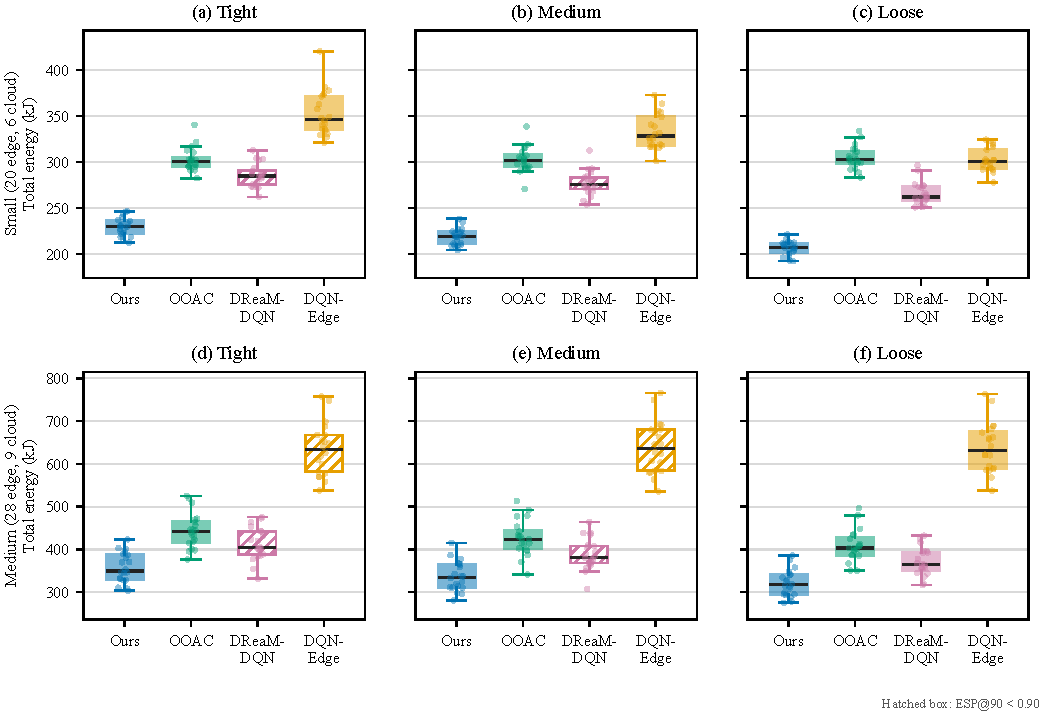
\includegraphics[width=0.98\textwidth]{figures/fig_energy_distributions.pdf}}{%
\fbox{\parbox[c][45mm][c]{0.9\textwidth}{\centering Energy-distribution figure placeholder}}}
\caption{Energy distributions on the fixed 20-seed test block. Energy should be compared only for methods that satisfy the ESP and reliability gates.}
\label{fig:energy_distributions}
\end{figure*}

\subsection{Workload--Resource Scalability}
We additionally form a balanced $2\times2$ workload--resource design. S26 and
M37 use base resources; S37 and M53 expand resources so the mean number of tasks
per server is approximately preserved. Every scenario uses a model trained for
its own exact state and action dimensions. Table~\ref{tab:scale_results} reports
our method and the strongest consistently feasible DVFS baseline, OOAC.

\begin{table*}[t]
\centering
\caption{Performance across workload--resource scales.}
\label{tab:scale_results}
\renewcommand{\arraystretch}{1.07}
\setlength{\tabcolsep}{6pt}
\resizebox{\textwidth}{!}{%
\begin{tabular}{@{}llrrrrrr@{}}
\toprule
& & \multicolumn{3}{c}{Proposed D3QN+SAC}
& \multicolumn{3}{c}{OOAC} \\
\cmidrule(lr){3-5}\cmidrule(lr){6-8}
Scenario & Deadline & Mean energy & Std. & ESP@90
& Mean energy & Std. & ESP@90 \\
\midrule
S26 & Loose  & \textbf{206.30} & 7.67 & 100\% & 304.56 & 12.50 & 100\% \\
    & Medium & \textbf{218.58} & 9.00 & 100\% & 302.31 & 13.71 & 100\% \\
    & Tight  & \textbf{229.67} & 9.71 & 100\% & 302.49 & 12.80 & 100\% \\
\cmidrule(lr){1-8}
S37 & Loose  & \textbf{121.57} & 6.02 & 100\% & 238.03 & 14.16 & 100\% \\
    & Medium & \textbf{132.07} & 7.42 & 100\% & 254.90 & 12.25 & 100\% \\
    & Tight  & \textbf{142.05} & 7.77 & 100\% & 266.43 & 13.77 & 100\% \\
\cmidrule(lr){1-8}
M37 & Loose  & \textbf{320.96} & 30.98 & 100\% & 409.02 & 37.22 & 100\% \\
    & Medium & \textbf{337.72} & 34.58 & 100\% & 426.94 & 41.54 & 100\% \\
    & Tight  & \textbf{357.54} & 35.11 & 95\% & 444.25 & 40.86 & 100\% \\
\cmidrule(lr){1-8}
M53 & Loose  & \textbf{309.98} & 30.49 & 100\% & 409.05 & 35.91 & 100\% \\
    & Medium & \textbf{337.16} & 39.20 & 90\% & 430.07 & 41.70 & 100\% \\
    & Tight  & \textbf{366.34} & 37.63 & 90\% & 445.62 & 44.09 & 100\% \\
\bottomrule
\end{tabular}}
\vspace{1mm}
\parbox{0.98\textwidth}{\footnotesize
Note: Energy is measured in kJ. S26 and S37 use small workflows with 26 and 37
servers; M37 and M53 use medium workflows with 37 and 53 servers. Bold denotes
the lower energy when both methods satisfy the 90\% ESP service threshold. All
reported reliability-attainment rates are 100\%.}
\end{table*}

Adding servers can increase total active energy even when contention falls,
because placement shifts toward faster or less energy-proportional server
profiles and more tasks execute concurrently. Therefore, server count alone is
not an energy monotonicity guarantee. The matched S37 and M53 models avoid the
invalid alternative of changing the action dimension of a previously trained
checkpoint. On the blind M53 block, the proposed method is strictly feasible
under loose deadlines and service-level feasible (90\% ESP) under medium and
tight deadlines. The post-hoc seed-replacement sensitivity analysis is excluded
from the formal results.

\subsection{Ablation Study}
Table~\ref{tab:ablation} isolates placement, DVFS, coordination, and the upper
deadline head on the small scenario. All trainable variants are selected without
using the final test block. The rows currently represent one training run per
variant and 20 evaluation seeds; they establish component behavior rather than
multi-training-seed optimization stability.

\begin{table*}[t]
\centering
\caption{Ablation results in the small workflow scenario.}
\label{tab:ablation}
\renewcommand{\arraystretch}{1.07}
\setlength{\tabcolsep}{6pt}
\resizebox{\textwidth}{!}{%
\begin{tabular}{@{}lrrrrrr@{}}
\toprule
& \multicolumn{2}{c}{Loose}
& \multicolumn{2}{c}{Medium}
& \multicolumn{2}{c}{Tight} \\
\cmidrule(lr){2-3}\cmidrule(lr){4-5}\cmidrule(lr){6-7}
Variant & Energy (kJ) & ESP@90 & Energy (kJ) & ESP@90
& Energy (kJ) & ESP@90 \\
\midrule
Full D3QN+SAC & \textbf{201.07$\pm$11.02} & 100\%
& \textbf{212.87$\pm$12.55} & 100\%
& \textbf{224.47$\pm$12.84} & 100\% \\
Full, fixed $\rho=1$ & 211.94$\pm$12.48 & 100\%
& 222.16$\pm$13.50 & 100\%
& 232.16$\pm$13.12 & 100\% \\
Independent upper, $\rho=1$ & 203.31$\pm$15.85 & 100\%
& 216.68$\pm$15.73 & 100\%
& 231.93$\pm$15.57 & 95\%$^{\dagger}$ \\
HEFT+SAC & 260.14$\pm$12.72 & 100\%
& 269.41$\pm$13.68 & 100\%
& 278.09$\pm$11.92 & 90\%$^{\dagger}$ \\
HEFT, fixed $\rho=1$ & 384.51$\pm$24.13 & 100\%
& 384.51$\pm$24.13 & 100\%
& 384.51$\pm$24.13 & 100\% \\
Without deadline head, $\rho=1$ & 48.46$\pm$1.81 & 0\%$^{\dagger}$
& 48.46$\pm$1.65 & 0\%$^{\dagger}$
& 48.49$\pm$1.66 & 0\%$^{\dagger}$ \\
\bottomrule
\end{tabular}}
\vspace{1mm}
\parbox{0.98\textwidth}{\footnotesize
Note: Energy is mean$\pm$standard deviation over 20 unseen seeds. Bold indicates
the lowest energy among variants meeting the ablation protocol's strict
ESP@90=100\% gate. The symbol $\dagger$ denotes a variant below this gate. All
variants achieve 100\% reliability attainment; the low energy without the
deadline head is infeasible and is not an energy improvement.}
\end{table*}

Using the same upper decisions, SAC reduces energy by 5.13\%, 4.18\%, and
3.31\% from loose to tight deadlines without losing feasibility. Relative to
HEFT+SAC, the full hierarchy saves 22.71\% and 20.99\% under loose and medium
deadlines. Under tight deadlines, HEFT+SAC reaches only 90\% ESP and therefore
is not a strict feasible energy competitor. Removing the upper deadline head
drives ESP to zero: its low energy reflects invalid placements rather than a
valid energy improvement. Finally, the independent upper policy loses strict
feasibility under tight deadlines, whereas the coordinated full method remains
at 100\%, supporting cross-level adaptation.

\subsection{Limitations}
Three limitations delimit the conclusions. First, the main reliability setting
is non-binding: every evaluated method reaches 100\% reliability attainment.
The reliability model and controller are retained for completeness, but a
separate benefit of the reliability head is not established. Second, the
ablation variants use one training seed; repeated training seeds are desirable
for optimization-stability claims. Third, the energy objective includes active
computation only. Idle-platform and communication energy should be added when
they are schedule-dependent in the target deployment.

\section{Conclusion}
\label{sec:conclusion}
This paper presented a constraint-aware hierarchical DRL method for dynamic
edge--cloud DAG scheduling. The upper three-head D3QN separates energy,
deadline, and reliability estimates for server placement, while the lower SAC
learns continuous DVFS. Queue-aware deadline credit, critical-path safety
features, episode failure feedback, and workflow counterfactual replay improve
the connection between delayed violations and their responsible decisions.
Under a constraint-first protocol, the method achieves 95--100\% ESP@90 and
100\% reliability attainment in the main scenarios while reducing energy
relative to feasible learning baselines. Future work will evaluate binding
reliability regimes, multiple independent training seeds, and energy models
that include idle and communication components.

\bibliographystyle{IEEEtran}
\bibliography{references}

\end{document}
